
% *** Authors should verify (and, if needed, correct) their LaTeX system  ***
% *** with the testflow diagnostic prior to trusting their LaTeX platform ***
% *** with production work. The IEEE's font choices and paper sizes can   ***
% *** trigger bugs that do not appear when using other class files.       ***                          ***
% The testflow support page is at:
% http://www.michaelshell.org/tex/testflow/

\documentclass[journal]{IEEEtran}
%
% If IEEEtran.cls has not been installed into the LaTeX system files,
% manually specify the path to it like:
% \documentclass[journal]{../sty/IEEEtran}

% Some very useful LaTeX packages include: (uncomment the ones you
% want to load)

\usepackage{enumitem,fancyhdr,setspace,float,soul,graphicx,
  epstopdf,multirow,sidecap,siunitx,
  amsmath,amsfonts,amsthm,amssymb,dsfont,booktabs,array,
  longtable,wrapfig,rotating,mathtools,xstring,
  textcomp,pdfpages,stackengine,lmodern}%
\usepackage[utf8]{inputenc}%
\usepackage[T1]{fontenc}%

\DeclareMathOperator{\E}{\mathbb{E}}%

\newcommand{\dd}[1]{\mathrm{d}#1}%
\newcommand\numberthis{\addtocounter{equation}{1}\tag{\theequation}}%
\newcommand{\sidenote}[1]{\textnormal{\textbf{(#1)}}}%
\newcommand{\norm}[1]{\left\lVert#1\right\rVert}%

\newtheorem{define}{Definition}[section]%
\newtheorem{prop}{Proposition}[section]%

\graphicspath{{figure/}}%

\usepackage{cite} \usepackage{amsmath}
% Note that the amsmath package sets \interdisplaylinepenalty to 10000
% thus preventing page breaks from occurring within multiline
% equations. Use:
\interdisplaylinepenalty=2500
% after loading amsmath to restore such page breaks as IEEEtran.cls
% normally does.

\usepackage{algorithm,algorithmic}

\ifCLASSOPTIONcompsoc
\usepackage[caption=false,font=normalsize,labelfont=sf,textfont=sf]{subfig}
\else \usepackage[caption=false,font=footnotesize]{subfig} \fi

\renewcommand{\algorithmicrequire}{\textbf{Input:}}
\renewcommand{\algorithmicensure}{\textbf{Output:}}
\renewcommand{\algorithmicrepeat}{\textbf{Iterate}}

% correct bad hyphenation here
\hyphenation{op-tical net-works semi-conduc-tor}


\begin{document}

\title{Parameters Inference of a 3D Solid Breast Texture Model from
  Clinical Data}

\author{Zhijin~Li, Ann-Katherine~Carton, Thomas~Almecija,
  Serge~Muller, Pablo~Milioni~de~Carlvalo and
  Agnès~Desolneux% <-this % stops a space
  \thanks{Zhijin Li is with General Electric Healthcare France, Buc,
    78530, France. E-mail:
    jonathan.li@ge.com.}% <-this % stops a space
  \thanks{Agnès Desolneux is with centre de math\'{e}matiques et leurs
    applications of Ecole Normale Sup\'{e}rieure de Paris-Sacaly,
    Cachan, 94235 France.}% <-this % stops a space
  \thanks{Ann-Katherine Carton, Thomas~Almecija, Serge Muller and
    Pablo~Milioni~de~Carlvalo are with General Electric Healthcare
    France, Buc, 78530, France.}% <-this % stops a space
  \thanks{Manuscript received December, XXXX; revised January XX,
    XXXX.}}

% The paper headers
\markboth{IEEE Transactions on Medical Imaging,~Vol.~14, No.~8,
  August~2017}%
{Shell \MakeLowercase{\textit{et al.}}: Bare Demo of IEEEtran.cls for
  IEEE Journals}
% The only time the second header will appear is for the odd numbered
% pages after the title page when using the twoside option.
%
% *** Note that you probably will NOT want to include the author's ***
% *** name in the headers of peer review papers.  *** You can use
% \ifCLASSOPTIONpeerreview for conditional compilation here if you
% desire.

% If you want to put a publisher's ID mark on the page you can do it
% like this: \IEEEpubid{0000--0000/00\$00.00~\copyright~2015 IEEE}
% Remember, if you use this you must call \IEEEpubidadjcol in the
% second column for its text to clear the IEEEpubid mark.

% use for special paper notices \IEEEspecialpapernotice{(Invited
% Paper)}

% make the title area
\maketitle

% As a general rule, do not put math, special symbols or citations in
% the abstract or keywords.
\begin{abstract}
  The abstract goes here.
\end{abstract}

% Note that keywords are not normally used for peerreview papers.
\begin{IEEEkeywords}
  X-ray breast imaging, virtual clinical trials, 3D breast texture
  model, stochastic geometry, statistical parameter inference.
\end{IEEEkeywords}

% For peer review papers, you can put extra information on the cover
% page as needed: \ifCLASSOPTIONpeerreview
% \begin{center} \bfseries EDICS Category: 3-BBND \end{center} \fi
%
% For peerreview papers, this IEEEtran command inserts a page break
% and creates the second title. It will be ignored for other modes.
\IEEEpeerreviewmaketitle

\section{Introduction and motivation}
\label{sec:intr-motiv}

% The very first letter is a 2 line initial drop letter followed by
% the rest of the first word in caps.
%
% form to use if the first word consists of a single letter:
% \IEEEPARstart{A}{demo} file is ....
%
% form to use if you need the single drop letter followed by normal
% text (unknown if ever used by the IEEE): \IEEEPARstart{A}{}demo file
% is ....
%
% Some journals put the first two words in caps: \IEEEPARstart{T}{his
% demo} file is ....
%
% Here we have the typical use of a "T" for an initial drop letter and
% "HIS" in caps to complete the first word.

\IEEEPARstart{C}{linical} trials are the ultimate way to assess the
performance of medical imaging systems. Due to their limitation by
cost and duration, several groups are investigating the potential to
replace clinical trials in part with virtual clinical trials (VCT) as
a more efficient alternative. In a reliable VCT study, a realistic
numerical 3D anthropomorphic test object, a realistic numerical image
acquisition chain and task-based observers are required. Today,
several numerical 3D anthropomorphic breast models have been proposed
\cite{li2009methodology} \cite{mahr2012three} \cite{carton2014virtual}
\cite{bakic2014realistic} \cite{chen2015description}
\cite{graff2016new} \cite{elangovan2017design}
\cite{sturgeon2017synthetic}. Each model presents advantages and
limitations in terms of the visual realism, statistical
characteristics and anatomical variability in model-simulated images
compared with clinical images. These aspects may impact the model
validity for certain performance assessment studies.

Previously, we proposed a mathematical 3D solid breast texture model
that is capable of simulating a large variability of realistic 2D and
3D breast images in terms of small and medium scale fibroglandular and
inter-glandular adipose tissue in breast \cite{li2016novel}. The
proposed model is inspired by the morphology and distribution of
medium and small scale fibroglandular and inter-glandular adipose
tissue observed in clinical breast computerized tomography (bCT)
reconstructed volumes. The reconstructed bCT volumes are stacks of
coronal slices reconstructed with a filtered back-projection algorithm
from projection images acquired using a prototype bCT system developed
at the University of California Davis Medical Center
\cite{lindfors2008dedicated}. The volumes were pre-processed by an
automatic 3D segmentation algorithm developed in-house to obtain
volumes depicting breast fibroglandular and adipose tissue
\cite{thomas2015segmentation}. Figure~\ref{fig:bct-ims} shows an
example of bCT reconstructed volume and its 3D segmentation. Our
proposed texture model aims to mimic the breast tissue characteristics
in segmented bCT volumes using mathematically defined stochastic
geoemtric elements.  For medium scale breast fibroglandular and
intra-glandular adipose tissue, we used a system of stochastically
distributed overlapping ellipsoids to depict the adipose compartments,
and the complement of the ellipsoid system to depict the
fibroglandular tissue. Small scale intra-glandular adipose compartment
irregularities were introduced by replacing the smooth ellipsoid
boundaries by Voronoi cells with average volume less than
\SI{1}{\mm\cubed}. The texture model outputs medium size rectangular
volumes in voxelized binary format, with typical side length between
\SI{3.5}{\cm} and \SI{5}{\cm}. Figure~\ref{fig:model} illustrates the
construction of the proposed texture model.

\begin{figure}[!htbp]
  \centering
  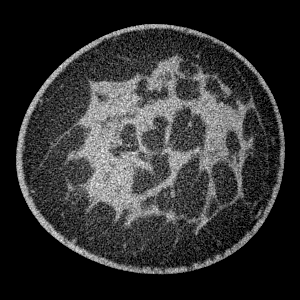
\includegraphics[width=0.145\textwidth]{gray-cor-small}%
  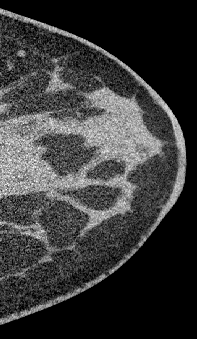
\includegraphics[height=0.145\textwidth]{gray-sag-small}%
  \hspace{2mm}%
  
\includegraphics[width=0.145\textwidth]{seg-cor-small}%
  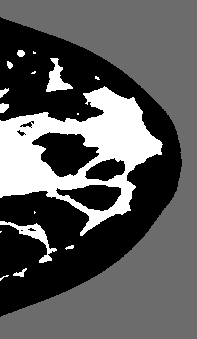
\includegraphics[height=0.145\textwidth]{seg-sag-small}

  \caption{Left: coronal and sagittal slices from an example of bCT
    reconstructed volumes. Right: coronal and sagittal slices from
    segmented volume of the same bCT volume, depicting fibroglandular
    tissue (white regions) and adipose tissue (black regions).}
  \label{fig:bct-ims}
\end{figure}

\begin{figure}[!htbp]
  \centering
  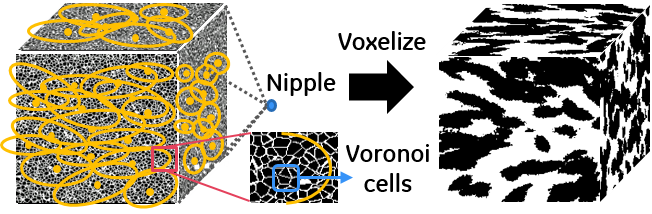
\includegraphics[width=0.4\textwidth]{model}
  \caption{Construction of our proposed 3D solid breast texture
    model. The medium intra-glandular adipose compartments are modeled
    by a system of random overlapping ellipsoids. Small scale
    intra-glandular adipose compartment irregularities were introduced
    by replacing the smooth ellipsoid boundaries by Voronoi cells. The
    texture model produces voxelized medium size rectangular binary
    volumes depicting fibroglandular tissue (white regions in the
    image on the right) and intra-glandular adipose tissue (black
    regions in the image on the right).}
  \label{fig:model}
\end{figure}

In our previous study, we proposed a prototype model implementation
with texture model parameters subjectively determined by visually
comparing the sampled texture volumes with reference bCT volumes. A
psycho-visual experiment was performed showing that the prototype
implementation was able to simulate realistic DBT reconstructed slices
representing a large variety of breast density types. However, further
observations show that the simulated DBT slices have a limited
morphological variability within each breast density type. This might
be due to the subjective model parameters, which might not correctly
capture the variability of breast tissue in clinical bCT volumes. To
allow the 3D solid breast texture model to simulate a larger
variability of breast textures, we propose to infer the model
parameters from clinical bCT volumes. A larger texture variability is
of interest in VCT studies, where the impact of various breast tissue
types on clinical task performance needs to be understood.

\section{Problem formulation}
\label{sec:problem-formulation}

We start by mathematically formulating the texture model and the
ground truth data. For this study, we focus on inferring the
medium scale model parameters related to the system of random
ellipsoids. The small scale parameters are not considered due to the
relatively low spatial resolution of the clinical bCT volumes, where
the voxel size is typically between \SI{0.2}{\mm} and
\SI{0.4}{\mm}. When the number of the small scale Voronoi cells is
large, the size of the cells may be in the same order of magnitude as
the voxel size in the bCT data. Therefore, the bCT data may not allow
for an accurate estimation of the small scale model parameters.

\subsection{The medium scale texture model}
\label{sec:medium-scale-texture}

The medium scale texture model is formulated as a \textit{marked point
  process} (MPP)
$$
\mathbf{Y} = \{ \mathbf{\Phi_{s}},\boldsymbol{\theta} \},
$$
defined on a product space
$S \subset \mathbb{R}^{3} \times \mathbb{R}^6$. Here,

\cite{chiu2013stochastic}.

\begin{itemize}

\item $\mathbf{\Phi_s}$ is a simple point process with distribution
  $\mathbf{P}^{\mathbf{s}}$. Its realization represents the center
  points of the ellipsoids.

\item $\boldsymbol{\theta}$ is a random vector with distribution
  $\mathbf{P}^{\boldsymbol{\theta}}$. Its realization represents the
  parameter vector of an ellipsoid. That is,
  $\boldsymbol{\theta} = \left( L_a, L_b, L_c, \delta_{\phi_a},
    \delta_{\phi_b}, \delta_{\phi_c} \right)$, where $L_a, L_b, L_c$
  are the half lengths of the principle axes of the ellipsoids and
  $\delta_{\phi_{x}},\delta_{\phi_{y}},\delta_{\phi_{z}}$ are random
  tilt angles. For each ellipsoid, the random tilt angles are added to
  three extrinsic rotation angles along $x$, $y$ and $z$ axes,
  determined by the center of the ellipsoid and the pre-defined nipple
  position. In marked point process theory, $\boldsymbol{\theta}$ is
  often referred to as the \textit{mark} of the point process
  $\mathbf{\Phi_s}$, and $\mathbf{P}^{\boldsymbol{\theta}}$ is often
  referred to as the \textit{mark distribution}
  \cite{chiu2013stochastic}.
\end{itemize}

\subsection{The ground truth}
\label{sec:ground-truth}

To limit the inference to the medium scale breast tissue, only volumes
of interest (VOI) with size \SI{3.5}{\cm} $\times$ \SI{3.5}{\cm}
$\times$ \SI{3.5}{\cm} of the segmented bCT volumes were
considered. The VOIs were extracted from the center of the segmented
bCT volumes, leaving at least \SI{2}{\cm} distance to the breast skin
and the chest-wall. None of the VOIs contained a lesion.

Mathematically, a segmented bCT VOI can be expressed as a binary
volume $\mathcal{D}$, where for any
$x \in \Omega \subset \mathbb{Z}^3$,
\begin{equation}
  \label{eq:bct-discrete-form}
  \mathcal{D}(x) =
  \begin{cases}
    1 & \textnormal{ if voxel } x \textnormal{ represents
      fibroglandular tissue}, \\
    0 & \textnormal{ if voxel } x \textnormal{ represents
      adipose tissue}. \\
  \end{cases}
\end{equation}
Here $\Omega$ represents the 3D discrete spatial domain of
$\mathcal{D}$.

Notice that, the input segmented clinical bCT VOIs depict adipose
compartments, where the individual ellipsoids are
\textit{unobservable}. This unobservability makes the inference problem
highly ill-posed.

\subsection{Existing methods}
\label{sec:exist-param-infer}

Due to the unobservability issue, application of
\textit{likelihood}-based parameter inference approaches
\cite{moller2003statistical} is impossible, since they require the
knowledge of the positions of the ellipsoid centers
\cite{dereudre2014estimation}. To mitigate this, one commonly used
approach in stochastic geometry is referred to as the \textit{minimum
  contrast estimator} (MCE) \cite{chiu2013stochastic}. Let
$\mathbf{\Theta}$ denote the set of all parameters for
$\mathbf{Y}$. The MCE method aims to find an estimate of
$\mathbf{\Theta}$ that minimizes a contrast function
$\mathcal{C}(\mathcal{D}, \mathbf{\Theta})$. The constrast function is
often expressed as the squared difference between some analytical
statistics of $\mathbf{Y}$ and the empirical counterparts of the
analytical statistics measured from the ground truth
$\mathcal{D}$. Popular choices of statistics include the two-point
function \cite{diggle1981binary} and the contact distribution function
\cite {heinrich1993asymptotic} etc. The major challenge of MCE is the
derivation of analytical summary statistics for complex underlying
model $\mathbf{Y}$. Considering the complexity of our input data,
application of MCE in our case might be non-trivial.

\section{Inference from reconstruction}
\label{sec:meth-infer-from}

Recently, Thiedmann \textit{et al.} proposed a novel inference method
for parametric MPP models that effectively mitigates the data
unobservability issue \cite{thiedmann2011stochastic}. Inspired by
their work, we hereby formally present this method and refer to it as
\textit{inference from reconstruction}. The method uses a two-step
approach. \textit{The first reconstruction step} aims at recovering
the unobserved point positions and marks from the observed data
through stochastic sampling. \textit{The second inference step} is a
parametric inference step where a marked point process model is fitted
to the reconstructed points and marks. This two-step mechanism
provides two main advantages over classical MCE method. First, once
the point positions and marks are recovered from the reconstruction
step, it is easier to perform statistical analysis to gain intuitions
to determine which model should be used for the inference
step. Second, the inference step using reconstructed point positions
and marks becomes more straightforward since all point positions are
observable. Due to these advantages, we decided to apply the inference
from reconstruction method to fit a parametric MPP model to the ground
truth segmented bCT data.

In the following section we describe in detail the methodology used
for the reconstruction step and the inference step in our study.

\subsection{The reconstruction step}
\label{sec:reconstr-step:-appr}

Consider the case where the density function $f_{\mathbf{Y}}$ of the
underlying MPP model $\mathbf{Y}$ has a Gibbsian form
\cite{moller2007modern}. Let
$\mathbf{u} = \{ \mathcal{E}_i\}_{i \in \mathbb{Z}} \subset S$ be a
finite set of ellipsoids, refered to as a configuration. Then we have:

\begin{equation}
  \label{eq:gibbs-density}
  f_{\mathbf{Y}}(\mathbf{u}) = \frac{1}{Z_T} \exp \left( - \frac{1}{T}
    E(\mathbf{u}) \right).
\end{equation}
Here the term $E(\cdot)$ is called the \textit{energy}. The parameter
$T \in \mathbb{R}^{+}$ is often referred to as the temperature as in
physics. The term
$Z_T = \int \exp \left( - \frac{E(\mathbf{u})}{T} \right) \dd
\mathbf{u}$ is a normalization constant. The energy term is often
decomposed into two parts \cite{lafarge2010geometric}
\cite{descombes2009object}:
\begin{equation}
  \label{mpp-energy}
  E(\mathbf{u}) = \mathcal{L}(\mathbf{u}, \mathcal{D})
  + \mathcal{P} (\mathbf{u}),
\end{equation}
where $\mathcal{L}(\mathbf{u}, \mathcal{D})$ is a \textit {data term}
representing how well a configuration $\mathbf{u}$ matches the ground
truth dataset $\mathcal{D}$; and $\mathcal{P} (\cdot)$ is a \textit
{prior term} containing the a-priori information of the underlying MPP
model $\mathbf{Y}$. Finding the best set of ellipsoids
$\mathbf{u}^{*}$ is equivalent to solving the following optimization
problem:
\begin{equation}
  \label{mpp-opt-energy}
  \mathbf{u}^{*}
  = \arg \max_{\mathbf{u}}{f_{\mathbf{Y}}(\mathbf{u})}
  = \arg\min_ {\mathbf{u}} \left( \mathcal{L}(\mathbf{u},
    \mathcal{D}) + \mathcal{P} (\mathbf{u}) \right).
\end{equation}

We formulated $\mathcal{L}(\mathbf{u}, \mathcal{D})$ and
$\mathcal{P} (\mathbf{u})$ as follows.

\begin{itemize}
\item
  Let $\mathcal{D}_{\mathbf{u}}$ be a discrete binary volume obtained
  by voxelizing a configuration $\mathbf{u}$ on the 3D discrete grid
  $\Omega$ defined in Section~\ref{sec:ground-truth}. Given a voxel
  $x \in \Omega$,
  \begin{equation}
    \label{eq:configuration-voxel}
    \mathcal{\mathcal{D}_{\mathbf{u}}}(x) =
    \begin{cases}
      1 & x\textnormal{'s center is inside an ellipsoid in }\mathbf{u}, \\
      0 & \textnormal{ otherwise}. \\
    \end{cases}
  \end{equation}
  Then $\mathcal{L}(\mathbf{u}, \mathcal{D})$ is formulated as
  \begin{equation}
    \label{eq:data-term1-single}
    % \mathcal{L}(\mathbf{u}, \mathcal{D}) = 1 - \frac{ 2 |
    % \neg \mathcal{D}_{\mathbf{u}} \wedge \neg \mathcal{D} |} {
    % |\neg \mathcal{D}_{\mathbf{u}} \vee \neg \mathcal{D}|},
    \mathcal{L}(\mathbf{u}, \mathcal{D}) = 1 - \frac{ |
      \{ x \in \Omega | \mathcal{D}_{\mathbf{u}}(x) = 0 \textnormal{
        and } \mathcal{D}(x) = 0 \} |} {
      |\{ x \in \Omega | \mathcal{D}_{\mathbf{u}}(x) = 0 \textnormal{
        or } \mathcal{D}(x) = 0 \}|},
  \end{equation}
  % where $|\cdot|$, $\wedge$ and $\vee$ denote the set cardinality,
  % logical conjunction, disjunction and negation respectively.

\item Regarding the \textit{prior term} $\mathcal{P} (\mathbf{u})$, we
  prefer to obtain a model estimate without imposing too much a-priori
  information on the distribution of the ellipsoids. Hence, only a
  weak constraint on the overlap ratio between ellipsoids is used to
  formulate $\mathcal{P} (\mathbf{u})$. That is:
  \begin{equation}
    \label{eq:prior-term}
    \mathcal{P} (\mathbf{u}) = \sum_{\mathcal{E} \in \mathbf{u}}
    q(\mathcal{E}, \mathbf{u} \setminus \mathcal{E}),
  \end{equation}
  where
  \begin{equation}
    \label{eq:prior-term-detail}
    q(\mathcal{E}, \mathbf{u} \setminus \mathcal{E}) =
    \begin{cases}
      0 & \textnormal{if }\frac{ | \{ x \in \Omega | x \in \mathcal{E}
        \textnormal{ and } x \in \mathbf{u} \setminus \mathcal{E} \}
        |} { | \{ x \in \Omega | x \in \mathcal{E} \} |}
      \le 0.95, \\
      +\infty & \textnormal{otherwise}.
    \end{cases}
  \end{equation}

\end{itemize}

The analytical solution of \eqref{mpp-opt-energy} is difficult to
obtain in pratice. In MPP literature, the \textit{reversible jump
  Markov chain Monte Carlo} (RJMCMC) sampling is a commonly employed
technique to tackle this type of optimization problem
\cite{descombes2013stochastic}. A typical RJMCMC procedure consists of
iteratively simulating a Markov chain of configurations
$\{ \mathbf{u}_t \}_{t \in \mathbb{N}}$ whose density converges to the
target density $f_{\mathbf{Y}}(\mathbf{u})$. At each iteration $t$, a
modification of the current configuration $\mathbf{u}_t$ is proposed
to create the next configuration $\mathbf{u}_{t+1}$. The term ``jump''
refers to the fact that the cardinality, \textit{i.e.} the number of
marked points of the current configuration might change during the
modification. A modification in RJMCMC is performed according to a
density function $Q(\mathbf{u}_t, \mathbf{u}_{t+1})$, referred to as a
proposition kernel. The modifications are local, in the sense that for
each iteration only one or two marked points in the current
configuration are modified. Typically, $Q(\mathbf{u}, \cdot)$ is a
combination of several sub-proposition kernels:
\begin{equation}
  \label{eq:sub-kernels}
  Q(\mathbf{u}, \cdot) = \sum_n p_n Q_n (\mathbf{u}, \cdot),
\end{equation}
where $p_n$ is the probability of the occurrence of the
sub-proposition kernels $Q_n(\cdot, \cdot)$, such that
$\sum_n p_n \le 1$ \cite{descombes2013stochastic}
\cite{verdie2014detecting}. Frequently investigated sub-proposition
kernels include:

\begin{itemize}

\item The \textit{Birth proposal}, in which a marked point is added to
  current configuration $\mathbf{u}_t$, according to a birth kernel
  denoted as $Q_{b}(\mathbf{u}, \cdot)$. That is,
  $\mathbf{u}_{t+1} = \mathbf{u}_t \cup \{u\}$, where $u$ is drawn
  according to $Q_{b}(\mathbf{u}, \cdot)$.

\item The \textit{Death proposal}. This is the reverse process of the
  birth proposal, in which a marked point is chosen and deleted from
  current configuration $\mathbf{u}$ according to a death kernel
  $Q_{d}(\mathbf{u}, \cdot)$. That is,
  $\mathbf{u}_{t+1} = \mathbf{u}_t \setminus \{u\}$, with
  $u \in \mathbf{u}_t$ chosen according to $Q_{d}(\mathbf{u}, \cdot)$.

  The combination of birth and death proposals ensures that the Markov
  chain is able to switch between configurations with different
  cardinality.

\item \textit{Perturbation proposal}. This proposal consists of
  changing the parametrization of a marked point $u$ in the current
  configuration $\mathbf{u}$ according to a perturbation kernel
  $Q_{p}(\mathbf{u}, \cdot)$.

\end{itemize}

In practice, the RJMCMC procedure might suffer from prohibitive rate
of convergence, since each iteration brings only one or two marked
points into play \cite{descombes2013stochastic}. To mitigate this
issue, a \textit{multiple births and deaths} algorithm has recently
been proposed by Descombes \textit{et al.} \cite{descombes2009object},
allowing for the births of multiple marked points at each iteration,
offering a more effective sampling procedure. In our study, we adapted
the multiple births and deaths algorithm design proposed in
\cite{descombes2009object}. For each iteration, the original multiple
births and deaths algorithm consisted of a birth step of multiple
marked points and a death step that examines all marked points in
current configuration. Additionally, to achieve a more effective
exploration of each configuration, we proposed to add an extra
perturbation step to the multiple births and deaths algorithm, named
as the \textit{shift} step.

To describe the shift step used in our adapted multiple births, deaths
and shifts (MBDS) algorithm, we adopt the notion of \textit{Legendre
  ellipsoid} of a convex body in classical mechanics
\cite{lutwak2000new}. Given a convex body $K \subset \mathbb{Z}^3$,
the Legendre ellipsoid $\mathcal{L}(K)$ is defined as
\cite{ludwig2003ellipsoids}:
\begin{equation}
  \label{eq:legendre-ellip-orig}
  \mathcal{L}(K) = \{ x \in K | x^T \Sigma^{-1} x \leq 1 \},
\end{equation}
where
\begin{equation}
  \label{eq:legendre-ellip-cov}
  \Sigma = \frac{\sum_{x \in K} (x - \mu)(x - \mu)^T} {|K|},
\end{equation}
with $\mu = \frac{1}{|K|} \sum_{x \in K} x$. Notice that
$\mathcal{L}(K) = K$ if $K$ is itself an ellipsoid.

Let $\mathcal{D}_{\mathcal{E}}$ be the binary volume representing
voxelized ellipsoid $\mathcal{E}$. The shift of $\mathcal{E}$ consists
in replacing it by the Legendre ellipsoid
$\mathcal{L}(K_{\mathcal{E}}(\mathcal{D}))$ of
$K_{\mathcal{E}}(\mathcal{D})$, with
\begin{equation}
  \label{eq:legendre-ellip}
  K_{\mathcal{E}}(\mathcal{D}) = \{x \in \Omega |
  \mathcal{D}(x) = 0 \textnormal{ and } \mathcal{D}_{\mathcal{E}}(x) = 0 \}.
\end{equation}

The complete description of the proposed MBDS algorithm is given by
Algorithm~\ref{algo-mbds}. We assumed that the proposal distribution
$f_{\boldsymbol{\theta}}$ consists of independent densities $f_{L_a}$,
$f_{L_b}$, $f_{L_c}$, $f_{\delta{\phi_1}}$, $f_{\delta{\phi_2}}$ and
$f_{\delta{\phi_3}}$ to sample the half lengths $L_a$, $L_b$, $L_c$
and the tilt angles $\delta{\phi_x}$, $\delta{\phi_y}$ of the
ellipsoids, $\delta{\phi_z}$. We set these densities to the ones used
in our previous study \cite{li2016novel}, since these previously
validated values might provide a good starting-point for the MBDS
algorithm and might accelerate the convergence of the algorithm.

\begin{algorithm}
  \caption{Multiple births, deaths and shifts}
  % \algsetup{indent=2em}
  \label{algo-mbds}
  \begin{algorithmic}[1]

    \REQUIRE initial configuration $\mathbf{u}_0 = \emptyset$,
    $T = 100$, $\mathbf{\Phi}$: a homogeneous Poisson point process
    with intensity $\lambda = 0.005$, $f_{\boldsymbol{\theta}}$: a
    multivariate proposal distribution to sample
    $ \left( L_a, L_b, L_c, \delta{\phi_1}, \delta{\phi_2},
      \delta{\phi_3} \right)$ and $\epsilon = 0.001$

    \ENSURE configuration $\mathbf{u}$

    \vspace{1mm} \REPEAT

    \vspace{1mm} \STATE \textbf{Multiple births}: sample configuration
    $u_b$ with ellipsoid centers $\sim \mathbf{\Phi}$, ellipsoid
    parameters $\sim f_{\boldsymbol{\theta}}$ \label{itr} \STATE
    $\mathbf{u} \rightarrow \mathbf{u} \cup u_b$

    \vspace{1mm} \STATE \textbf{Deaths and shifts}:

    \FOR{$\mathcal{E} \in \mathbf{u}$} \STATE
    $p_d = \frac{r\lambda}{1 + r\lambda}$ with
    $r = \exp \left( \frac{ E(\mathbf{u}) - E(\mathbf{u} \setminus
        \mathcal{E}) }{T} \right)$ and $E(\cdot)$ given in
    \eqref{mpp-energy}

    \STATE Sample $v \sim \textnormal{uniform}(0, 1)$

    \IF{$v < p_d$} \STATE
    $\mathbf{u} \rightarrow \mathbf{u} \setminus \mathcal{E}$ \ELSE
    \STATE
    $\mathcal{E} \rightarrow
    \mathcal{L(K_{\mathcal{E}(\mathcal{D})})}$ with
    $\mathcal{L}(\cdot)$ given in \eqref{eq:legendre-ellip-orig}.
    \ENDIF

    \ENDFOR

    \vspace{1mm} \STATE \textbf{Update}:
    $\lambda \rightarrow \lambda \cdot 0.99 \textnormal{ and } T
    \rightarrow T \cdot 0.99$

    \vspace{1mm} \STATE \textbf{Convergence test}: collect 10
    consecutive energies $c_t = \{E_{t-9}, E_{t-8}, \cdots, E_{t}\}$
    up to current iteration $t$

    \IF{$\max \left( c_t \right) - \min \left( c_t \right) \le
      \epsilon$} \STATE \textbf{return} configuration $\mathbf{u}$
    \ELSE \STATE \textbf{continue}
    \ENDIF

    \UNTIL{\textbf{return}}
  \end{algorithmic}
\end{algorithm}

\setcounter{table}{0}

\subsection{The inference step}
\label{sec:infer-step:-fitt}

Once a segmented bCT VOI is represented as a system of ellipsoids with
known spatial positions and shape parameters, we fit a parametric MPP
model to the reconstructed ellipsoids. To reduce the complexity of the
inference step, we assume in the first instance that the marks of the
MPP model are independent from each other and that they are
independent from the ellipsoid centers. This allows us to fit the
center point process of the ellipsoids and their shape parameters
separately.

\subsubsection{The point process for reconstructed ellipsoid centers}
\label{sec:point-proc-reconstr}

To gain some intuition on the type of point process model
$\mathbf{\Phi_s}$ for the fit, we first analyzed the \textit{pair
  correlation function} (PCF) of the reconstructed ellipsoid centers
for each ground truth data set. The PCF is a commonly studied
second-order statistical descriptor in stochastic geometry that can
help reveal comprehensive structural information of a point process
\cite{baddeley2007spatial}.

\begin{define}

  The pair correlation function \textit{$g(\cdot, \cdot)$} of a simple
  point process $\mathbf{\Phi}$ with intensity function
  $\lambda(\cdot)$ is defined as:
  \begin{equation}
    \label{eq:pcf-official-def}
    g(x,y)=\frac{\rho^{(2)}(x,y)}{\lambda(x) \lambda(y)}.
  \end{equation}
  Here $\rho^{(2)}(\cdot, \cdot)$ is the second order moment density
  of $\mathbf{\Phi}$, satisfying
  \begin{equation}
    \label{eq:second-order-moment}
    \int_{B_{1} \times B_{2}} \rho^{(2)}(x,y) \, \dd x \dd y
    = \sum^{x \neq y}_{x,y \in \mathbf{\Phi}} \E \left( \mathds{1} (
      \{x,y \} \in B_{1} \times B_{2} ) \right),
  \end{equation}
  for arbitrary bounded Borel sets $B_1$ and $B_2$.
\end{define}

The PCF can be used to interpret the interaction between points in a
point process \cite{illian2008statistical}. For all Poisson processes
where there are no interactions between points, $g(x,y)=1$. If
$g(x,y)>1$, an \textit{attraction} between points at locations $x$ and
$y$ exists. If $g(x,y)<1$, a \textit{repulsion} between points at
locations $x$ and $y$ exists.

In our study, we assumed that the centers of the reconstructed
ellipsoids come from a stationary and isotropic point process. This
indicates that the PCF depends only on the relative distance between
two spatial positions. That is, $g(x, y) = g(r)$, where
$r = \norm{x-y}$ is referred to as the \textit{interpoint
  distance}. Under this assumption, we applied the PCF estimator
described in \cite[p232]{illian2008statistical} to estimate the
empirical PCF of reconstructed ellipsoid centers from each segmented
bCT VOI. Analytically, the PCF estimator is expressed as:
\begin{equation}
  \label{eq:pcf-estimator}
  \hat{g}(r; \Phi_s) = \sum^{x \neq y}_{x, y \in \Phi_s \cap W}
  \frac{\mathbf{k}(\norm{x-y} - r)}
  {4 \pi r^2 \nu(W_x \cap W_y) \hat{\lambda}^2},
\end{equation}
where $\Phi_s$ is the collection of all ellipsoid centers
reconstructed from a dataset and $\hat{\lambda}$ is an estimate of its
intensity parameter, expressed as
\begin{equation}
  \label{eq:inten-estimtor}
  \hat{\lambda} = \frac{|\Phi_s|}{\nu(W)}.
\end{equation}
The function $\mathbf{k}(\cdot)$ is a smoothing kernel. We use
$\nu(\cdot)$ to denote the volume measure and $W$ is the observation
window; \textit{i.e.} a \SI{3.5}{\cm} $\times$ \SI{3.5}{\cm} $\times$
\SI{3.5}{\cm} cube in our case. Finally, $W_x$ denotes the translation
of $W$ by $x$. The division by $\nu(W_x \cap W_y)$ instead of by
$\nu(W)$ acts as an edge correction for points falling outside of the
observation window $W$ \cite{ohser1983estimators}.

The estimation was performed using the \texttt{pcf3est} function
implemented in the \texttt{R} software package \texttt{spatstat}
\cite{baddeley2005spatstat} with its default setting. In this setting
the \textit{Epanechnikov} smoothing kernel \cite{chiu2013stochastic}
was used. Mathematically, the \textit{Epanechnikov} kernel is defined
as:
\begin{equation}
  \label{eq:epan-kernel}
  \mathbf{k}(s) =
  \begin{cases}
    \frac{3}{4\delta} (1 - \frac{s^2}{\delta^2}) & \textnormal{if }
    -\delta \leq s \leq \delta, \\
    0 & \textnormal{ otherwise}.
  \end{cases}
\end{equation}
It has a bandwidth parameter $\delta$ to tune. In the default setting
of \texttt{pcf3est}, $\delta$ is set according to the rule-of-thumb:
$\delta = \frac{0.26}{\sqrt[3]{\hat{\lambda}}}$
\cite{baddeley2005spatstat}.

Once the empirical estimates of PCFs were obtained, we first checked
if the Poisson property can or can not be rejected based on the PCF
estimates. This check was performed using the envelope test described
in~\cite{baddeley2014tests}. We will show in
Section~\ref{sec:inference-step} that the analysis of the PCFs
revealed a clustering interaction between reconstructed ellipsoid
centers for the majority of the cases. To model the clustering
interaction, we proposed to fit a three-dimensional \textit{Mat\'ern
  cluster process} \cite{baddeley2007spatial} to the reconstructed
ellipsoid centers.

The 3D Mat\'ern cluster process is a two-step process. First, a set of
``parent points'' $\{ y_i \}_{i \in \mathcal{I}} \subset \mathbb{R}^3$
are sampled from a homogeneous Poisson point process with intensity
parameter $\kappa$. For each ``parent point'' $y_i$ with
$i \in \mathcal{I}$, a sphere with radius $R$ centered at $y_i$ is
generated. Then, inside each obtained sphere, a set of ``children
points'' are sampled from another homogeneous Poisson point process
with intensity parameter $\lambda_0$. A realization of the Mat\'ern
cluster process is obtained as the collection of all ``children
points''.

A Mat\'ern cluster process model $\Phi_\mathcal{M}$ is a stationary
and isotropic point process completely determined by the three
parameters: $\kappa$, $\lambda_0$, and $R$. Theoretical formula for
the PCF of a 3D Mat\'ern cluster process is analytically accessible
and is given by the following proposition
\cite[p376]{illian2008statistical}.

\begin{prop}
  Let $\Phi_{\mathcal{M}}$ be a Mat\'ern cluster process with
  parameters $\kappa, \lambda, R$, then its intensity parameter
  $\lambda$ is:
  \begin{equation}
    \label{eq:matern-inten}
    \lambda = \frac{4}{3}\pi R^3\kappa \lambda_0.
  \end{equation}
  Its pair correlation function $g$ is:
  \begin{equation}
    \label{eq:matern-pcf}
    g(r; \kappa, \lambda_0, R) =
    \begin{cases}
      1 + \frac{3(R - \frac{r}{2})^2 (2R + \frac{r}{2})} {8\pi \kappa
        R^6}
      & \textnormal{if } 0 < r \leq 2R, \\
      1 & \textnormal{if } r > 2R. \\
    \end{cases}
  \end{equation}
\end{prop}

To fit a Mat\'ern cluster process with parameters $\kappa, \lambda, R$
to a set of reconstructed ellipsoid centers $\Phi_s$, we applied the
MCE method described in Section~\ref{sec:exist-param-infer}. For a
given $\Phi_s$, the contrast function $\mathcal{C}$ was computed based
on the analytical and empirical PCF. That is,
\begin{equation}
  \label{eq:matern-contrast}
  \mathcal{C}(r; \kappa, \lambda_0, R, \Phi_s) =
  \sum_{r \in \mathcal{R}} (g(r; \kappa, \lambda_0, R) -
  \hat{g}(r; \Phi_s))^2,
\end{equation}
where $\hat{g}(r, \Phi_s)$ is given in \eqref{eq:pcf-estimator} and
$g(r; \kappa, \lambda_0, R)$ is given in \eqref{eq:matern-pcf}. Here
$\mathcal{R}$ denotes the set of interpoint distances considered by
the MCE estimator. Additionally, \eqref{eq:matern-inten} was used as
an equality constraint. Let
$\mathbf{\Theta} = \left( \kappa, \lambda_0, R \right)$, for a given
set of reconstructed ellipsoids $\Phi_s$, the MCE estimator
$\widehat{\mathbf{\Theta}}$ is formally expressed as:
\begin{equation}
  \label{eq:mce-est-complete}
  \begin{aligned}
    \widehat{\mathbf{\Theta}} & = \arg \min_{\mathbf{\Theta}} \sum_{r
      \in \mathcal{R}} \left( g(r; \kappa, \lambda_0, R)
      - \hat{g}(r; \Phi_s) \right)^2, \\
    & \textnormal{subjected to: } \hat{\lambda} = \frac{4}{3}\pi
    R^3\kappa \lambda_0.
  \end{aligned}
\end{equation}

The optimization \eqref{eq:mce-est-complete} was numerically solved
using the function \texttt{fmincon} implemented in the \texttt{Matlab}
software (version \texttt{2016b}, The MathWorks Inc., Natick,
Massachusetts, United States). The default setting of \texttt{fmincon}
was used. In this setting, the \textit{interior point} optimization
method is applied, with the Hessian of the contrast function
$\mathcal{C}(\cdot)$ approximated using the \textit{Broyden\textendash
  Fletcher\textendash Goldfarb\textendash Shanno} algorithm. We set
$\mathcal{R}$ to be a set of values increasing from \SI{0.2}{\mm} to
\SI{30}{\mm} with a step size of \SI{0.2}{\mm}. All optimizations were
run with an initial condition $\kappa = 0.1$, $\lambda_0 = 0.1$ and
$R = 1$. The convergence was considered reached when the contrast
function was non-decreasing in all feasible directions, within the a
tolerance value of \num{1e-6}. Since we were able to obtain fairly
good fit for all input datasets
(Section~\ref{sec:point-proc-reconstr}), the impact of different
configurations of the optimization function was considered
out-of-scope in our study and was not investigated.

\subsubsection{The mark distribution}
\label{sec:mark-distribution}

Empirical statistics of each individual mark were examined separately
from the ellipsoid centers. Histograms of the half lengths $L_a$,
$L_b$, $L_c$ and the tilts angles $\delta\phi_x$, $\delta\phi_y$,
$\delta\phi_z$ of the reconstructed ellipsoids were obtained to
visualize the empirical distributions of $L_a$, $L_b$ and $L_c$. Based
on the empirical statistical analysis, independent distributions were
proposed for each mark.

% An example of a floating figure using the graphicx package.  Note
% that \label must occur AFTER (or within) \caption.  For
% figures, \caption should occur after the \includegraphics.  Note
% that IEEEtran v1.7 and later has special internal code that is
% designed to preserve the operation of \label within \caption even
% when the captionsoff option is in effect. However, because of issues
% like this, it may be the safest practice to put all your
% \label just after \caption rather than within \caption{}.
      %
% Reminder: the "draftcls" or "draftclsnofoot", not "draft", class
% option should be used if it is desired that the figures are to be
% displayed while in draft mode.
      %
      %       \begin{figure}[!t]
      %         \centering
      %         \includegraphics[width=2.5in]{myfigure}
      %         where an .eps filename suffix will be assumed under
      %         latex, and a
      %         .pdf suffix will be assumed for pdflatex; or what has
      %         been declared
      %         via \DeclareGraphicsExtensions.
      %         \caption{Simulation results for the network.}
      %         \label{fig_sim}
      %       \end{figure}

      %       Note that the IEEE typically puts floats only at the
      %       top, even when
      %       this results in a large percentage of a column being
      %       occupied by
      %       floats.


      %       An example of a double column floating figure using two
      %       subfigures.
      %       (The subfig.sty package must be loaded for this to
      %       work.)  The
      %       subfigure \label commands are set within each subfloat
      %       command, and
      %       the \label for the overall figure must come
      %       after \caption.  \hfil
      %       is used as a separator to get equal spacing.  Watch out
      %       that the
      %       combined width of all the subfigures on a line do not
      %       exceed the
      %       text width or a line break will occur.
      %
      %       \begin{figure*}[!t]
      %         \centering \subfloat[Case
      %         I]{\includegraphics[width=2.5in]{box}%
      %         \label{fig_first_case}} \hfil \subfloat[Case
      %         II]{\includegraphics[width=2.5in]{box}%
      %         \label{fig_second_case}}
      %         \caption{Simulation results for the network.}
      %         \label{fig_sim}
      %       \end{figure*}
      %
      %       Note that often IEEE papers with subfigures do not
      %       employ subfigure
      %       captions (using the optional argument to \subfloat[]),
      %       but instead
      %       will reference/describe all of them (a), (b), etc.,
      %       within the main
      %       caption.  Be aware that for subfig.sty to generate the
      %       (a), (b),
      %       etc., subfigure labels, the optional argument to
      %       \subfloat must be
      %       present. If a subcaption is not desired, just leave its
      %       contents
      %       blank, e.g., \subfloat[].


      %       An example of a floating table. Note that, for IEEE
      %       style tables,
      %       the
      %       \caption command should come BEFORE the table and, given
      %       that table
      %       captions serve much like titles, are usually capitalized
      %       except for
      %       words such as a, an, and, as, at, but, by, for, in, nor,
      %       of, on, or,
      %       the, to and up, which are usually not capitalized unless
      %       they are
      %       the first or last word of the caption. Table text will
      %       default to
      %       \footnotesize as the IEEE normally uses this smaller
      %       font for
      %       tables.  The \label must come after \caption as always.
      %
      %       \begin{table}[!t]
      %%         increase table row spacing, adjust to taste
      %         \renewcommand{\arraystretch}{1.3} if using array.sty,
      %         it might be
      %         a good idea to tweak the value of \extrarowheight as
      %         needed to
      %         properly center the text within the cells
      %         \caption{An Example of a Table}
      %         \label{table_example}
      %         \centering
      %%         Some packages, such as MDW tools, offer better
      %%         commands for
      %%         making tables than the plain LaTeX2e tabular which is
      %%         used here.
      %         \begin{tabular}{|c||c|}
      %       \hline
      %       One & Two\\
      %               %       \hline
      %               %       Three & Four\\
      %               %       \hline
      %       \end{tabular}
      %     \end{table}


      %     Note that the IEEE does not put floats in the very first
      %     column - or
      %     typically anywhere on the first page for that
      %     matter. Also, in-text
      %     middle ("here") positioning is typically not used, but it
      %     is allowed
      %     and encouraged for Computer Society conferences (but not
      %     Computer
      %     Society journals). Most IEEE journals/conferences use top
      %     floats
      %     exclusively.  Note that, LaTeX2e, unlike IEEE
      %     journals/conferences,
      %     places footnotes above bottom floats. This can be
      %     corrected via the
      %     \fnbelowfloat command of the stfloats package.

\section{Results}
\label{sec:results}

We performed parameter inference on a collection of 16 sets of
segmented clinical bCT VOIs. The selected VOIs have BI-RADS densities
(5th Edition, \cite{d2013acr}) that cover category a, b and c, and
represent a considerable variability in medium scale fibroglandular
and inter-glandular adipose breast tissue. In this section, we
demonstrate the results focusing on examples of three bCT VOIs,
referred to as VOI \#1, \#2 and \#3, with glandular densities
belonging to BI-RADS density category a, b and c respectively.

\subsection{The reconstruction step}
\label{sec:reconstruction-step}

Figure~\ref{fig:conv-mbds} shows the decrease of the energy with the
increasing number of iterations for the three bCT VOIs. We can see
that the convergence was reached after about 7500 iterations for all
the cases. Similar results were obtained for other investigated bCT
VOIs.

\begin{figure}[!htb]
  \centering
  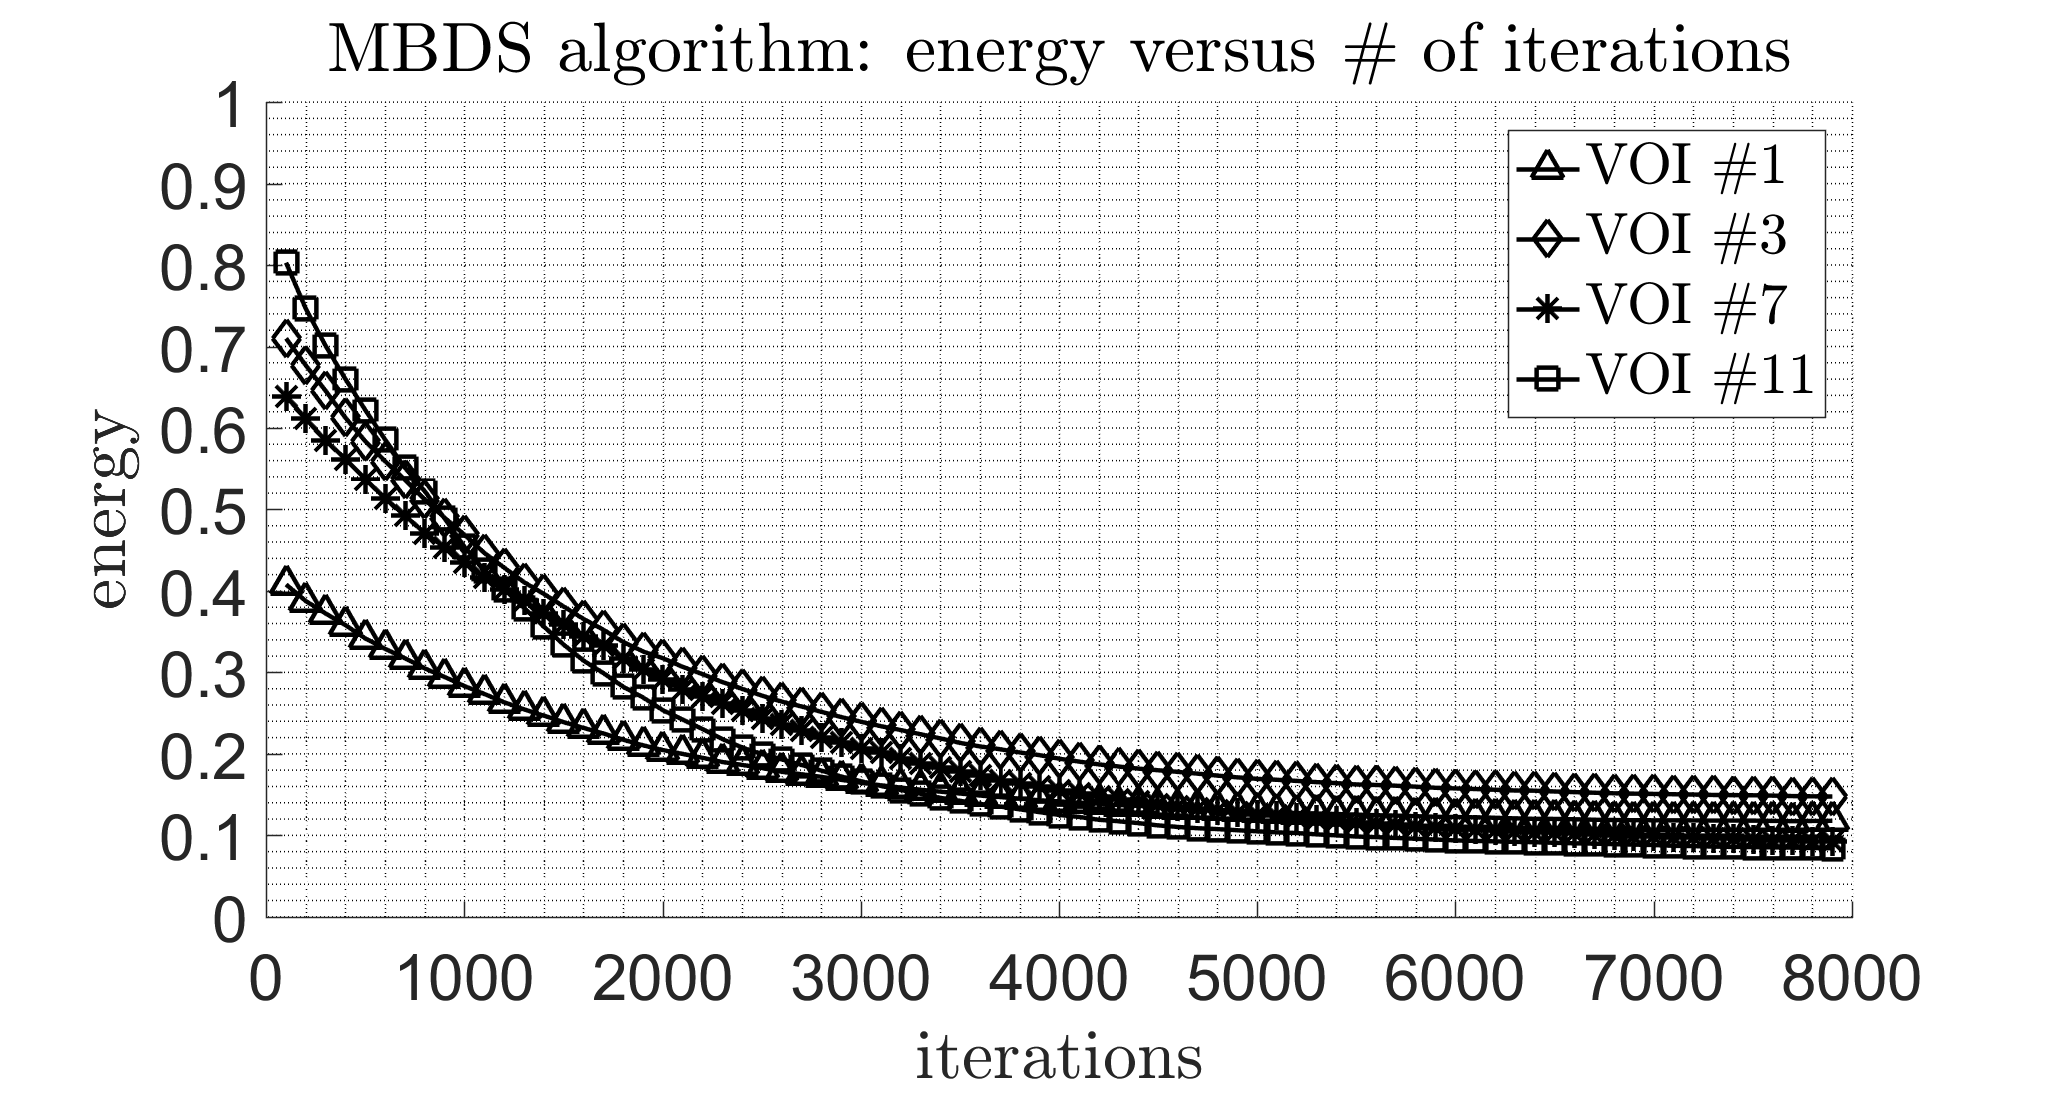
\includegraphics[width=0.5\textwidth]
  {figure/convergence_mbds}
  \caption{Illustration of the energy defined in~\eqref{mpp-energy} as
    a function of the number of iterations in the MBDS algorithm for
    VOI \#1, VOI \#2 and VOI \#3. The convergence of the MBDS
    algorithm was reached after about 7500 iterations for all the
    cases.}
  \label{fig:conv-mbds}
\end{figure}

The result of the reconstruction step for VOI \#1, \#2 and \#3 is
demonstrated in Figure~\ref{fig:bct-datasets-recon} by comparing the
original VOIs with the reconstructed VOIs. Reconstructed VOIs are
binary volumes having the same spatial and voxel size as their
corresponding bCT VOIs. They were created by voxelizing the
reconstructed ellipsoids from the MBDS algorithm and assigning value 0
to the ellipsoid interior. Projection images of the original VOIs and
the reconstructed VOIs are also demonstrated. The projections were
obtained by averaging the VOIs in the direction perpendicular to the
transverse plane.

From Figure~\ref{fig:bct-datasets-recon} we can see that the
reconstructions by ellipsoids are not perfect. Despite this, the
distribution and morphology of the medium scale fibroglandular and
inter-glandular adipose tissue in reconstructed VOIs agree fairly well
with the original segmented clinical bCT VOIs. Also, the medium scale
texture variations in the projections of the original VOIs are
preserved in the projections of the reconstructed VOIs. The result of
the reconstruction step provides sufficiently good input for follow-up
inference step.

\begin{figure}[!htb]

  \centering
  \captionsetup[subfloat]{labelformat=empty}

  {\fontsize{9}{9}\selectfont VOI \#1} \vspace{1mm}

  \raisebox{0.5em}{\fontsize{9}{9}\selectfont \rotatebox{90}{Ground
      truth}}
  
\includegraphics[width=0.14\textwidth]
  {figure/all/dataset_3/roi_coronal}
  
\includegraphics[width=0.14\textwidth]
  {figure/all/dataset_3/roi_saggital}
  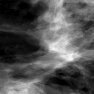
\includegraphics[width=0.14\textwidth]
  {figure/all/dataset_3/proj_roi}

  \raisebox{0.5em}{\fontsize{9}{9}\selectfont
    \rotatebox{90}{Reconstruction}}
  
\includegraphics[width=0.14\textwidth]
  {figure/all/dataset_3/model_coronal}
  
\includegraphics[width=0.14\textwidth]
  {figure/all/dataset_3/model_saggital}
  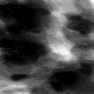
\includegraphics[width=0.14\textwidth]
  {figure/all/dataset_3/proj_roi_inten10}

  {\fontsize{9}{9}\selectfont VOI \#2} \vspace{1mm}

  \raisebox{0.5em}{\fontsize{9}{9}\selectfont \rotatebox{90}{Ground
      truth}}
  
\includegraphics[width=0.14\textwidth]
  {figure/all/dataset_7/roi_coronal}
  
\includegraphics[width=0.14\textwidth]
  {figure/all/dataset_7/roi_saggital}
  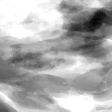
\includegraphics[width=0.14\textwidth]
  {figure/all/dataset_7/proj_roi}

  \raisebox{0.5em}{\fontsize{9}{9}\selectfont
    \rotatebox{90}{Reconstruction}}
  
\includegraphics[width=0.14\textwidth]
  {figure/all/dataset_7/model_coronal}
  
\includegraphics[width=0.14\textwidth]
  {figure/all/dataset_7/model_saggital}
  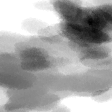
\includegraphics[width=0.14\textwidth]
  {figure/all/dataset_7/proj_roi_inten10}

  {\fontsize{9}{9}\selectfont VOI \#3} \vspace{1mm}

  \raisebox{0.7em}{\fontsize{9}{9}\selectfont \rotatebox{90}{Ground
      truth}}
  
\includegraphics[width=0.14\textwidth]
  {figure/all/dataset_11/roi_coronal}
  
\includegraphics[width=0.14\textwidth]
  {figure/all/dataset_11/roi_saggital}
  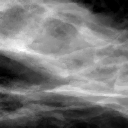
\includegraphics[width=0.14\textwidth]
  {figure/all/dataset_11/proj_roi}

  \raisebox{1.1em}{\fontsize{9}{9}\selectfont
    \rotatebox{90}{Reconstruction}}
  \stackon{\fontsize{9}{9}\selectfont
    Coronal}{
\includegraphics[width=0.14\textwidth]
    {figure/all/dataset_11/model_coronal}}
  \stackon{\fontsize{9}{9}\selectfont
    Saggital}{
\includegraphics[width=0.14\textwidth]
    {figure/all/dataset_11/model_saggital}}
  \stackon{\fontsize{9}{9}\selectfont
    Projection}{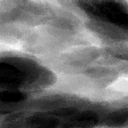
\includegraphics[width=0.14\textwidth]
    {figure/all/dataset_11/proj_roi_inten10}}

  \caption{Illustration of coronal slices, saggital slices and
    projections of VOIs \#1, \#2, \#3, and their reconstructed
    VOIs. The sizes of the VOIs are \SI{3.5}{\cm} $\times$
    \SI{3.5}{\cm} $\times$ \SI{3.5}{\cm}. Reconstructed VOIs are
    binary volumes with the same size and resolution as their
    corresponding segmented clinical bCT VOIs. They were created by
    voxelizing the reconstructed ellipsoids from the MBDS algorithm
    and assigning value 0 to the ellipsoid interior. Projections
    images were obtained by averaging the VOIs in the direction
    perpendicular to the transverse plane. The distribution and
    morphology of the medium scale fibroglandular and inter-glandular
    adipose tissue in reconstructed VOIs agree fairly well with the
    original segmented clinical bCT VOIs}
  \label{fig:bct-datasets-recon}

\end{figure}

\subsection{The inference step}
\label{sec:inference-step}

By analyzing the estimated PCFs of the reconstructed ellipsoid centers
from the 16 input bCT VOIs using the envelope test method described in
\cite{baddeley2014tests}, we found that for four VOIs, the Poisson
null-hypothesis can not be rejected. For the remainder of our study,
these VOIs were excluded since they represented a much smaller
population among all bCT VOIs.

The three figures on the left in Figure~\ref{fig:pcf-est} compare the
empirical PCFs estimated from the reconstructed ellipsoid centers for
VOI \#1, \#2, \#3 and the theoretical Poisson PCFs. The envelopes of
the Poisson PCFs generated using the method described in
\cite{baddeley2014tests} are also shown. Figure~\ref{fig:pcf-est}
indicates that the empirical PCFs estimated from the reconstructed
ellipsoid centers of the three VOIs exhibit a clustering effect. This
can be seen if we look at the interpoint distance $r = $ \SI{3}{\mm}
emphasized in Figure~\ref{fig:pcf-est}. The envelope test rejects the
null-hypothesis for all demonstrated VOIs at $r = $ \SI{3}{\mm}. The
same clustering effect was found for all other investigated bCT VOIs.

\begin{figure}[!htb]
  \centering

  \captionsetup[subfloat]{labelformat=empty,position=top}

  \subfloat[VOI \#1]{\includegraphics[width=0.24\textwidth]%
    {figure/all/dataset_3/pcf_new}%
    \includegraphics[width=0.24\textwidth]%
    {figure/all/dataset_3/fit_pcf_matern}}%

  \subfloat[VOI \#2]{\includegraphics[width=0.24\textwidth]%
    {figure/all/dataset_7/pcf_new}%
    \includegraphics[width=0.24\textwidth]%
    {figure/all/dataset_7/fit_pcf_matern}}%

  \subfloat[VOI \#3]{\includegraphics[width=0.24\textwidth]%
    {figure/all/dataset_11/pcf_new}%
    \includegraphics[width=0.24\textwidth]%
    {figure/all/dataset_11/fit_pcf_matern}}%

  \caption{Figures on the left compare the empirical PCFs (dashed
    lines) estimated from the reconstructed ellipsoid centers for VOI
    \#1, \#2, \#3 and the theoretical Poisson PCFs (solid lines). Gray
    surfaces are the envelopes of the Poisson PCFs generated using the
    method described in \cite{baddeley2014tests}. The envelope test
    rejects the Poisson null-hypothesis for all four VOIs at
    interpoint distance $r = $ \SI{3}{\mm}. Figures on the right
    compares the same empirical PCFs and the theoretical PCFs (solid
    lines) of the Mat\'ern cluster processes fitted to the same
    VOIs. Gray surfaces are the envelopes of the PCFs of the fitted
    Mat\'ern cluster processes generated using the method described in
    \cite{baddeley2014tests}. The empirical PCFs fall inside the
    envelopes at all interpoint distances, indicating good fits.}
  \label{fig:pcf-est}

\end{figure}

\subsubsection{Parameters of the 3D Mat\'ern cluster process}
\label{sec:parameters-3d-matern}

The three figures on the right in Figure~\ref{fig:pcf-est} compare the
empirical PCFs estimated from the reconstructed ellipsoid centers for
VOI \#1, \#2, \#3 and the theoretical PCFs of the Mat\'ern cluster
processes fitted to the same VOIs. The PCF envelopes of the fitted
Mat\'ern cluster processes were also generated using the method
described in \cite{baddeley2014tests}, but with the fitted Mat\'ern
cluster process as the null hypothesis model. It can be seen that for
the three VOIs, the the empirically estimated PCFs fall inside the
envelopes at all interpoint distances. Based on this, we conclude that
the fits are fairly good. Similar result was found for all other
investigated bCT VOIs.

\subsubsection{The mark distribution}
\label{sec:mark-distribution-1}

Figure~\ref{fig:ellip-axes-distr} shows the histograms of the half
lengths $L_a$, $L_b$, $L_c$ and the tilt angles $\delta\phi_x$,
$\delta\phi_y$, $\delta\phi_z$ of the reconstructed ellipsoids for VOI
\#1, \#2 and \#3. From visual observations, we notice that the
distributions of $L_a$, $L_b$, $L_c$, $\delta\phi_y$ and
$\delta\phi_z$ seem to be Gaussian and the distribution of
$\delta\phi_x$ seems to be uniform between $-\frac{\pi}{2}$ and
$\frac{\pi}{2}$. Similar observations were also obtained for
reconstructed ellipsoids from other bCT VOIs. Following these
observations, we then fitted the distributions of $L_a$, $L_b$, $L_c$,
$\delta\phi_y$ and $\delta\phi_z$ to Gaussian distributions using the
maximum likelihood estimator. A series of Kolmogorov-Smirnov tests
were also performed to verify the statistical validity of the fit. The
tests show that for more 80\% of the cases, the fit was good
statistically under 5\% confidence interval.

\begin{figure}[!htb]
  \centering

  \captionsetup[subfloat]{labelformat=empty,position=top}

  \subfloat[VOI \#1]{\includegraphics[width=0.24\textwidth]%
    {figure/all/dataset_3/axes_distr_new_small}%
    \includegraphics[width=0.24\textwidth]%
    {figure/all/dataset_3/tilts_distr_new_small}}%

  \subfloat[VOI \#2]{\includegraphics[width=0.24\textwidth]%
    {figure/all/dataset_7/axes_distr_new_small}%
    \includegraphics[width=0.24\textwidth]%
    {figure/all/dataset_7/tilts_distr_new_small}}%

  \subfloat[VOI \#3]{\includegraphics[width=0.24\textwidth]%
    {figure/all/dataset_11/axes_distr_new_small}%
    \includegraphics[width=0.24\textwidth]%
    {figure/all/dataset_11/tilts_distr_new_small}}%

  \caption{Histograms of the half lengths $L_a$, $L_b$, $L_c$ and the
    tilt angles $\delta\phi_x$, $\delta\phi_y$, $\delta\phi_z$ of
    reconstructed ellipsoids for VOI \#1, \#2 and \#3. Visual
    observations show that these parameters seem to follow either
    Gaussian or uniform distributions.}
  \label{fig:ellip-axes-distr}
\end{figure}

As a summary, Table~\ref{tab:summary-inferred-params} lists the fitted
medium scale parameters for VOI \#1, \#2 and \#3. By applying the
inference from reconstruction method to all the 12 input bCT VOIs, 12
new sets of medium scale parameters were finally obtained.

\begin{table}[!htb]
  {\fontsize{9}{8}\selectfont
    \begin{center}

      \caption{Medium scale parameters for the 3D stochastic breast
        texture model fitted from VOIs \#1, \#2 and \#3. Here
        $\mathcal{N}(\mu, \sigma)$ denotes the Gaussian distribution
        with mean $\mu$, standard deviation $\sigma$; and
        $\mathcal{U}(l,u)$ denotes the uniform distribution with lower
        bound $l$ and upper bound $u$.}

      \begin{tabular}{ m{1.6cm} m{1.8cm} m{1.8cm} m{1.8cm} }

        \toprule

        \centering{\textbf{Parameters}}
        & \centering{VOI \#1}
        & \centering{VOI \#2}
        & \centering{VOI \#3}
          \tabularnewline%\\

        \cmidrule(lr){1-1} \cmidrule(lr){2-2}
        \cmidrule(lr){3-3} \cmidrule(lr){4-4}

        \centering{$\kappa$ (\si{\per\mm\cubed})}
        & \centering{$3.24e-03$}
        & \centering{$3.41e-03$}
        & \centering{$2.87e-04$}
          \tabularnewline%\\

        \cmidrule(lr){1-1} \cmidrule(lr){2-2}
        \cmidrule(lr){3-3} \cmidrule(lr){4-4}

        \centering{$\lambda_0$ (\si{\per\mm\cubed})}
        & \centering{$5.98e-03$}
        & \centering{$1.92e-02$}
        & \centering{$3.09e-02$}
          \tabularnewline%\\

        \cmidrule(lr){1-1} \cmidrule(lr){2-2}
        \cmidrule(lr){3-3} \cmidrule(lr){4-4}

        \centering{$R$ (\si{\mm})}
        & \centering{$5.98$}
        & \centering{$3.85$}
        & \centering{$5.82$}
          \tabularnewline%\\

        \cmidrule(lr){1-1} \cmidrule(lr){2-2}
        \cmidrule(lr){3-3} \cmidrule(lr){4-4}

        \centering{$p_{L_a}$ (\si{\mm})}
        & \centering{$\mathcal{N}(6.21, 1.41)$}
        & \centering{$\mathcal{N}(5.88, 1.44)$}
        & \centering{$\mathcal{N}(6.06, 1.39)$}
          \tabularnewline%\\

        \cmidrule(lr){1-1} \cmidrule(lr){2-2}
        \cmidrule(lr){3-3} \cmidrule(lr){4-4}

        \centering{$p_{L_b}$ (\si{\mm})}
        & \centering{$\mathcal{N}(2.77, 0.58)$}
        & \centering{$\mathcal{N}(2.75, 0.56)$}
        & \centering{$\mathcal{N}(2.79, 0.56)$}
          \tabularnewline%\\

        \cmidrule(lr){1-1} \cmidrule(lr){2-2}
        \cmidrule(lr){3-3} \cmidrule(lr){4-4}

        \centering{$p_{L_c}$ (\si{\mm})}
        & \centering{$\mathcal{N}(2.10, 0.57)$}
        & \centering{$\mathcal{N}(2.03, 0.52)$}
        & \centering{$\mathcal{N}(2.10, 0.54)$}
          \tabularnewline%\\

        \cmidrule(lr){1-1} \cmidrule(lr){2-2}
        \cmidrule(lr){3-3} \cmidrule(lr){4-4}

        \centering{$p_{\delta_{\phi_x}}$ (\si{\radian})}
        & \centering{$\mathcal{U}(-\frac{\pi}{2}, \frac{\pi}{2})$}
        & \centering{$\mathcal{U}(-\frac{\pi}{2}, \frac{\pi}{2})$}
        & \centering{$\mathcal{U}(-\frac{\pi}{2}, \frac{\pi}{2})$}
          \tabularnewline%\\

        \cmidrule(lr){1-1} \cmidrule(lr){2-2}
        \cmidrule(lr){3-3} \cmidrule(lr){4-4}

        \centering{$p_{\delta_{\phi_y}}$ (\si{\radian})}
        & \centering{$\mathcal{N}(-0.09, 0.4)$}
        & \centering{$\mathcal{N}(-0.15, 0.38)$}
        & \centering{$\mathcal{N}(-0.28, 0.47)$}
          \tabularnewline%\\

        \cmidrule(lr){1-1} \cmidrule(lr){2-2}
        \cmidrule(lr){3-3} \cmidrule(lr){4-4}

        \centering{$p_{\delta_{\phi_z}}$ (\si{\radian})}
        & \centering{$\mathcal{N}(0, 0.26)$}
        & \centering{$\mathcal{N}(0.01, 0.5)$}
        & \centering{$\mathcal{N}(-0.01, 0.43)$}
          \tabularnewline%\\

        \bottomrule

      \end{tabular}

      \label{tab:summary-inferred-params}
    \end{center}
  }
\end{table}


\section{Validation of inferred medium scale texture model parameters}
\label{sec:valid-inferr-medi}

\subsection{Visual inspection}
\label{sec:visual-validation-1}

To visually inspect the realism of simulated x-ray breast images using
the fitted medium scale texture model parameters, a simulation
experiment was conducted. Three texture volumes were simulated using
respectively the three set of medium scale parameters listed in
Table~\ref{tab:summary-inferred-params}. The average size of the small
Voronoi cells was set to be \SI{0.1}{\mm\cubed}. The nipple position
and the voxel size for each volume were set to be the same as in the
corresponding ground truth bCT data. Mammograms and DBT projection
images were simulated by virtually projecting the texture volumes
using the previously described breast x-ray imaging simulator
\cite{milioni2014low}. The x-ray simulator was adjusted to model the
topology of the GE SenoClaire DBT imaging system. A mono-energetic
x-ray source at \SI{20}{\keV} was used to simulate nine DBT projection
images with an angular range of $( \ang{-12.5}, \ang{12.5} )$. Only
Poisson x-ray noise was modeled as the noise source. X-ray scattering
and blurring on the detector were not modeled. The size of the
isotropic detector pixels is \SI{100}{\um}. Mechanical breast texture
deformation to mimic breast compression during the DBT image
acquisition was not modeled. Projection images were processed by the
\texttt{ASIR-DBT} 3D reconstruction algorithm (GE Healthcare, Buc,
France) to obtain DBT reconstructed slices with \SI{1}{\mm} slice
thickness.

Figure~\ref{fig:fit-params-sims} shows examples of \SI{3.5}{\cm}
$\times$ \SI{3.5}{\cm} slices through the simulated texture volumes,
as well as mammographic projections and DBT reconstructed slices
simulated from these volumes. Visual inspection of the simulated
images indicates fairly high visual realism. Also, compared with
images simulated using the prototype implementation
\cite{li2016novel}, the new model parameters are capable of simulating
mammographic projections and and DBT reconstructed slices with a
larger morphological variability. These observations indicate an
improvement of the model's realism and morphological variability
compared with the prototype implementation with empirical parameters
proposed in the previous chapter.

\begin{figure}[!htb]
  \centering

  \hspace{1mm} \parbox{2.8cm}{\fontsize{9}{9}\selectfont \centering
    Texture volumes slices} \parbox{2.8cm}{\fontsize{9}{9}\selectfont
    \centering Mammographic
    projections} \parbox{2.75cm}{\fontsize{9}{9}\selectfont \centering
    DBT reconstructed slices} \vspace{1mm}

  \raisebox{3em}{\fontsize{9}{9}\selectfont \rotatebox{90}{VOI \#1}}
  
\includegraphics[width=0.15\textwidth]
  {figure/all/dataset_3/sim_vol_small}
  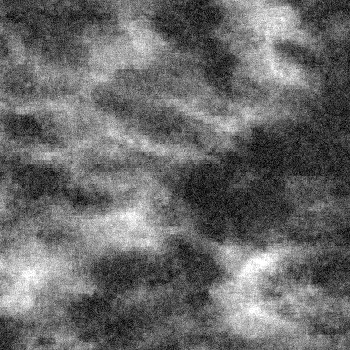
\includegraphics[width=0.15\textwidth]
  {figure/all/dataset_3/sim_proj}
  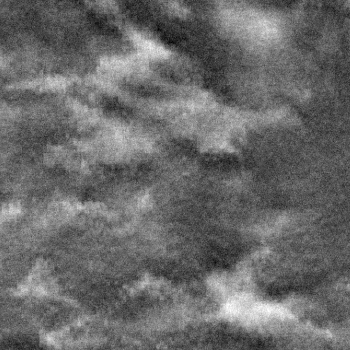
\includegraphics[width=0.15\textwidth]
  {figure/all/dataset_3/sim_recon}

  \raisebox{3em}{\fontsize{9}{9}\selectfont \rotatebox{90}{VOI \#2}}
  
\includegraphics[width=0.15\textwidth]
  {figure/all/dataset_7/sim_vol_small}
  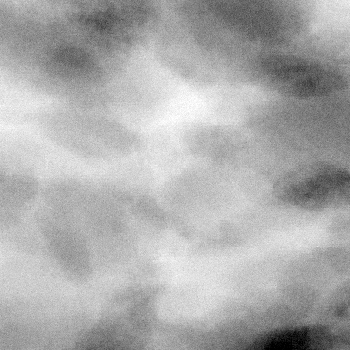
\includegraphics[width=0.15\textwidth]
  {figure/all/dataset_7/sim_proj}
  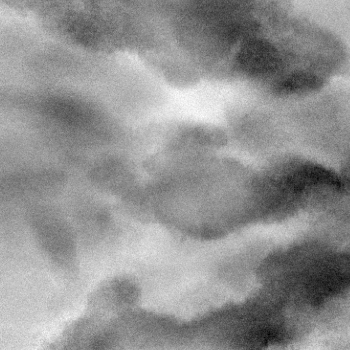
\includegraphics[width=0.15\textwidth]
  {figure/all/dataset_7/sim_recon}

  \raisebox{3em}{\fontsize{9}{9}\selectfont \rotatebox{90}{VOI \#3}}
  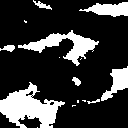
\includegraphics[width=0.15\textwidth]
  {figure/all/dataset_11/sim_vol_small}
  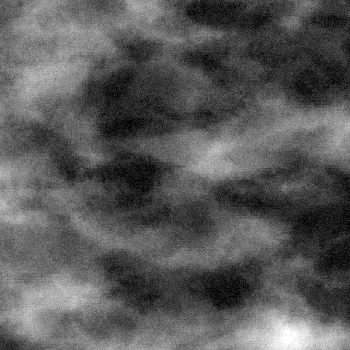
\includegraphics[width=0.15\textwidth]
  {figure/all/dataset_11/sim_proj}
  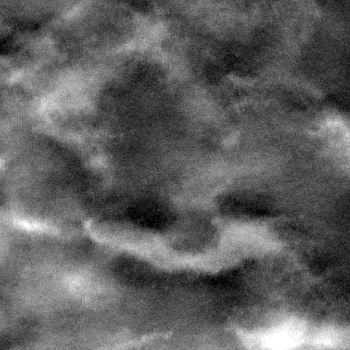
\includegraphics[width=0.15\textwidth]
  {figure/all/dataset_11/sim_recon}

  \caption{The first column shows slices through volumes simulated
    from the 3D breast texture model with the four sets of parameters
    listed in Table~\ref{tab:summary-inferred-params}. The second
    column shows mammographic projections simulated from the simulated
    texture volumes. The third column shows DBT reconstructed slices
    simulated from the simulated texture volumes. The sizes of the
    images are \SI{3.5}{\cm} $\times$ \SI{3.5}{\cm}.}
  \label{fig:fit-params-sims}
\end{figure}

\subsection{Statistical validation}
\label{sec:stat-valid}

As a statistical validation of the realism of simulated breast images
using the new model parameters, we performed statistical estimations
of the $\beta$ metric on simulated breast images. The $\beta$ metric
measures the inverse slope of the log-scale noise power spectrum (NPS)
of an image and is the most commonly used statistical metric for the
realism of simulated breast images. For each of the obtained 12 sets
of medium model parameters, 100 texture volumes were simulated under
the same set-up as described in the previous section. From each
simulated texture volume, \SI{3.5}{\cm} $\times$ \SI{3.5}{\cm}
mammographic projection and DBT reconstructed slices were obtained
using the same x-ray simulator and 3D reconstruction algorithm as
described in previous section. We used the method described by Wu
\textit{et al.} \cite{wu2012spectral} to estimate the $\beta$ values
from the mammographic projection and central DBT slices. In this
method, each input image was first divided into \SI{2.5}{\cm} $\times$
\SI{2.5}{\cm} regions of interest (ROI) with 50\% overlap. Then the
ROIs were multiplied by a Hann window and their average power spectrum
was used as the NPS estimate. Finally, a linear regression of the NPS
versus the frequency in log scale was performed within a frequency
range of $\left[ \SI{0.1}{\per\mm}, \SI{0.7}{\per\mm} \right]$, and
the inverse of the regression slope was used as the $\beta$
estimate. We found that the $\beta$ values of the simulated
mammography projections have an average of XXX and a standard
deviation of XXX; the $\beta$ values of the simulated DBT central
slices have an average of XXX and a standard deviation of XXX. These
values are consistent with those reported in literature [REFERENCE].

\subsection{Psycho-visual validation}
\label{sec:psych-valid-valid}

A two-alternative forced choice (2AFC) experiment was performed to
formally assess the visual realism of simulated DBT reconstructed
images. Pairs of 3.5 $\times$ \SI{3.5}{\cm\squared} ROIs, extracted
from images simulated from our texture model and clinical bCT data
were displayed side-by-side. Images on the left always came from the
clinical bCT data set, while images on the right had 50\% chance to be
from the texture model and 50\% chance to be from clinical bCT
data. The reader had to tell whether the image on the right was from
the clinical bCT data set or from the texture model. Similar level of
glandular density was maintained for each image pair. In total, 144
image pairs were presented; 52 pairs from BI-RADS density category a,
56 pairs from BI-RADS density category b and 36 pairs from BI-RADS
density category c. Images were displayed on 5M pixels grayscale
portrait monitors (SMD 21500 G, Siemens AG; Munchen, Germany) at 100\%
resolution. Each image pair was displayed during 5 seconds, followed
by the display of a uniform gray–level image for another 5 seconds;
the readers were thus imposed to make a decision within 10
seconds. Four readers participated in the experiment, all GE
Healthcare engineers. Reader 1, 2 and 3 have no prior knowledge of our
texture model while reader 4 knows the algorithm of the texture model
construction. A short training session with 10 image pairs of known
ground truth was performed before the real experiment with no time
constraint. The reading distance was set to be one meter. The
percentage of correct answers, $P_c$, was calculated as an indication
for the realism of the simulated images from the texture model. Under
the null hypothesis that images simulated from the model and clinical
bCT images data cannot be distinguished, $P_c = 0.5$.

TO BE MODIFIED [The left chart of Figure 5 shows the Pc value of the
four readers of the 2AFC experi-ments. Readers 1 and 2 had overall Pc
values of 0.65 and 0.66, while reader 3 had a Pc value of 0.73
indicating that he could more easily distinguish texture images from
clinical bCT images. Reader 4 had the highest Pc value of 0.82. He
reported that he was able to infer simulated images from his prior
knowledge of the intermediate steps of the model construction. Readers
1, 3 and 4 reported that they had observed a quantification effect
appearing like “small square blocks” in some simulated images from the
texture model, as illustrated in the right image of Figure 5. When
this effect was present, they used it as criterion to distinguish
simulated images using the texture model from those using clinical bCT
data. Reader 2 did not report the same primary criteria. This ‘small
square block artifact’ can likely be attributed to the size of the
Voronoi cells at the transition of glandular/adipose tissue. Table 2
reports Pc for each reader by type of breast density. The p-value
indicates whether the reader was or was not able to differentiate
simulated data from real data. The lower Pc values for al-most
entirely adipose breasts can be explained by the lower number of
adipose/dense transitions, designed by Voronoi cells, in this type of
breasts.]

\section{Conclusion and discussion}
\label{sec:concl-disc}

In this paper, we investigated the inference of the medium scale
parameters of a previously introduced 3D solid breast texture model
from clinical breast computerized tomography (bCT) reconstructed
volumes of interest (VOI), to improve the anatomical variability for
virtual clinical trials. We applied a novel two-step inference method
referred to as the inference from reconstruction.

From the majority of the bCT VOIs, a clustering effect between
ellipsoids was observed and was further modeled using a 3D Mat\'{e}rn
cluster process. Twelve sets of new medium scale model parameters were
obtained. Visual evaluation of the 2D and 3D breast images simulated
from 3D texture volumes generated using new parameters shows fairly
high visual realism. The morphological variability in new simulated
images is larger than the images simulated using previously proposed
prototype implementation with empirical parameters. The values of the
$\beta$ metric measure from simulated mammographic projections and DBT
slices are consistent with values reported in literature. Finally, a
formal two-alternative forced choice experiment involving XXXX readers
was performed. The experimental results demonstrated that the model
with inferred parameters can simulate realistic DBT reconstructed images
for breasts with BI-RADS density categories a, b and c.

The proposed method has several limitations. First, the impact of the
reconstruction step on the estimated parameters in the inference step
was not investigated. To address this, one possible approach is to
study the inference stability with respect to an analytically known
ground truth model such as a Poisson marked point process. Second, to
reduce the optimization complexity in the inference step, the
distribution of ellipsoid half lengths were estimated independently
from the ellipsoid centers. This may be a simplification compared with
the distribution of inter-glandular adipose compartments in real
breasts. The correlation between the the half lengths and the centers
of the ellipsoids could be further investigated by studying the mark
correlation function of the reconstructed ellipsoids. Finally, we
obtained twelve separate sets of model parameters from twelve
different input bCT VOIs. In a future study, it might be interesting
to model how the model parameters change with respect to the BI-RADS
density of the input, in order to create a unified model.

% A multiple births, deaths and shifts (MBDS) algorithm was employed
% to first reconstruct a set of random ellipsoids from each ground
% truth bCT VOI. Visual inspection of the volumes recreated by
% voxelizing the reconstructed ellipsoids shows a fairly good
% approximation of the medium scale breast tissue in the original bCT
% VOIs. A Mat\'{e}rn cluster process was then fitted to the
% reconstructed ellipsoid centers using the minimum contrast method
% based on the pair correlation functions (PCF). This introduces a
% clustering interaction between ellipsoids to the previous prototype
% model. Statistical diagnostic analysis using the PCF suggested a
% fairly good fit of the reconstructed ellipsoid centers to the
% proposed Mat\'{e}rn cluster process. Distributions of the ellipsoid
% half lengths and orientations were finally estimated from their
% empirical distributions. Twelve sets of new medium scale model
% parameters were obtained.


% if have a single appendix:
% \appendix[Proof of the Zonklar Equations]
% or
% \appendix % for no appendix heading
% do not use \section anymore after \appendix, only \section* is
% possibly needed

% use appendices with more than one appendix then use \section to
% start each appendix you must declare a \section before using any
% \subsection or using \label (\appendices by itself starts a section
% numbered zero.)
        %

% use section* for acknowledgment
\section*{Acknowledgment}

This research is partially funded by the French national association
for research and technology (ANRT) under the CIFRE grant n\textdegree
2013/1052. The authors would like to thank Prof. John Boone for kindly
providing the clinical bCT data sets.


% Can use something like this to put references on a page by
% themselves when using endfloat and the captionsoff option.
\ifCLASSOPTIONcaptionsoff
\newpage
\fi



% trigger a \newpage just before the given reference number - used to
% balance the columns on the last page adjust value as needed - may
% need to be readjusted if the document is modified later
% \IEEEtriggeratref{8} The "triggered" command can be changed if
% desired: \IEEEtriggercmd{\enlargethispage{-5in}}

% references section

% can use a bibliography generated by BibTeX as a .bbl file BibTeX
% documentation can be easily obtained at:
% http://mirror.ctan.org/biblio/bibtex/contrib/doc/ The IEEEtran
% BibTeX style support page is at:
% http://www.michaelshell.org/tex/ieeetran/bibtex/
% \bibliographystyle{IEEEtran} argument is your BibTeX string
% definitions and bibliography database(s)
% \bibliography{IEEEabrv,../bib/paper}
        %
% <OR> manually copy in the resultant .bbl file set second argument
% of \begin to the number of references (used to reserve space for the
%   reference number labels box)

%   \begin{thebibliography}{1}

%   \bibitem{IEEEhowto:kopka} H.~Kopka and P.~W. Daly, \emph{A Guide
%     to \LaTeX}, 3rd~ed.\hskip 1em plus 0.5em minus 0.4em\relax
%     Harlow, England: Addison-Wesley, 1999.

%   \end{thebibliography}

\bibliography{biblio/biblio} \bibliographystyle{ieeetr}


% that's all folks
\end{document}


%%% Local Variables:
%%% mode: latex
%%% TeX-master: t
%%% End:
